\documentclass[a4paper, 11pt]{article}


\usepackage{amsmath}
\usepackage{amssymb}
\usepackage[unicode]{hyperref}
\usepackage{url}
\usepackage{a4wide}
\usepackage[utf8]{inputenc}
\usepackage[main = russian, english]{babel}
\usepackage[pdftex]{graphicx}
\usepackage{float}
\usepackage{subcaption}
\usepackage{indentfirst}

%% TIKZ
\usepackage{tikz}                % Векторная графика
								 %
\usepackage{pgfplots}            % % Нужно для вставки графиков из 
\pgfplotsset{compat=newest}      % % matlab2tikz
\usetikzlibrary{plotmarks}       % %
\usetikzlibrary{arrows.meta}     % %
\usepgfplotslibrary{patchplots}  % %
\usepackage{grffile}             % %

\newcommand{\R}{\mathbb{R}}
\newcommand{\N}{\mathbb{N}}

\begin{document}
	\thispagestyle{empty}
\begin{center}
    \ \vspace{-3cm}

    \includegraphics[width=0.5\textwidth]{title_page/msu.eps}\\

    {\scshape Московский государственный университет имени М.~В.~Ломоносова}\\
    Факультет вычислительной математики и кибернетики\\
    Кафедра системного анализа

    \vfill

    {\LARGE Практикум}

    \vspace{1cm}
    {\Huge\bfseries <<Волновые решения в \\распределённой модели ``хищник--жертва''>>}
\end{center}

\vspace{3cm}

\begin{flushright}
    \large
    \textit{Студент 515 группы}\\
    К.\,Ю.~Егоров

    \vspace{5mm}

    \textit{Руководитель практикума}\\
    д.ф.-м.н., профессор Д.\,А.~Алимов
\end{flushright}

\vfill

\begin{center}
    Москва, 2020
\end{center}

\clearpage
	\tableofcontents
	\clearpage
	
	\section{Постановка задачи}
	Рассматривается двумерная динамическая система
	\begin{equation}\label{eq:basic-task}
		\left\{\begin{aligned}
			\dot u &= \frac{au(K - u)}{K} - \frac{buv}{1+Nu} + d_1 u_{xx} \\
			\dot v &= -cv + \frac{duv}{1 + Nu} +d_2 v_{xx},
		\end{aligned}\right.
	\end{equation}
	где $a$, $b$, $c$, $d$, $N$, $K$, $d_1$, $d_2$~--- положительные параметры, $(u,\,v) \in \R^2_{+}$.
	Здесь $u(x,t)$ ($v(x,t))$~--- плотность популяции жертв (хищников) в точке с координатой $x$ в момент времени $t$, $t > 0$, $x \in \R$, $d_1,\,d_2$~--- величины коэффициентов диффузии жертв и хищников соответственно.

	В рамках задачи, для системы \eqref{eq:basic-task} требуется:
	\begin{enumerate}
		\item Уменьшить число параметров, сделав замену переменных;
		\item Исследовать фазовый портрет нераспределённой системы;
		\item Проверить наличие решений распределённой системы;
		\item Выбрать подходящее решение и скорость волны;
		\item Привести иллюстрации и графики фазовых портретов и решений.
	\end{enumerate}


	\section{Уменьшение числа параметров}
	Для уменьшения числа параметров проведём линейную замену переменных, которая не изменит свойств исходной системы. Итак, пусть
	$$
		\tilde u = \alpha u, \;
		\tilde v = \beta v,  \;
		\tilde t = \gamma t, \;
		\tilde x = \delta x.
	$$
	Тогда частные производные исходных переменных $u$ и $v$ примут вид:
	$$
		u_t = \frac{\partial}{\partial t} \left(\frac{\tilde u}{\alpha}\right) =
		\frac{\gamma}{\alpha}\tilde u_{\tilde t},
		\quad
		u_x = \frac{\partial}{\partial x} \left(\frac{\tilde u}{\alpha}\right) =
		\frac{\delta}{\alpha}\tilde u_{\tilde x},
		\quad
		u_{xx} = \frac{\delta^2}{\alpha}\tilde u_{\tilde x \tilde x},
	$$
	$$
		v_t = \frac{\partial}{\partial t} \left(\frac{\tilde v}{\beta}\right) =
		\frac{\gamma}{\beta}\tilde v_{\tilde t},
		\quad
		v_x = \frac{\partial}{\partial x} \left(\frac{\tilde v}{\beta}\right) =
		\frac{\delta}{\beta}\tilde v_{\tilde x},
		\quad
		v_{xx} = \frac{\delta^2}{\beta}\tilde v_{\tilde x \tilde x}.
	$$
	Подстановкой в рассматриваемую систему \eqref{eq:basic-task} получим
	\begin{equation}\label{eq:changed-system}
		\left\{\begin{aligned}
			\frac{\gamma}{\alpha} \tilde u_{\tilde t} =&
			\frac{a}{\alpha K}\tilde u(K - \tilde u) -
			\frac{b}{\alpha\beta}\cdot\frac{\tilde u \tilde v}{1 + \frac{N}{\alpha}\tilde u} +
			\frac{d_1 \delta^2}{\alpha} \tilde u_{\tilde x \tilde x}\\
			\frac{\gamma}{\beta} \tilde v_{\tilde t} =&
			-\frac{c}{\beta} \tilde v +
			\frac{d}{\alpha\beta}\cdot\frac{\tilde u \tilde v}{1 + \frac{N}{\alpha}\tilde u} +
			\frac{d_2 \delta^2}{\beta} \tilde v_{\tilde x \tilde x}.
		\end{aligned}\right.
	\end{equation}

	Заметим, что если выбрать коэффициенты замены таким образом:
	$$
		\alpha = N,\; \beta = \frac{Nb}{d},\;
		\gamma = \frac{d}{N}, \delta^2 = \frac{d}{d_1 N},
	$$
	то система \eqref{eq:changed-system} примет вид
	\begin{equation}
		\left\{\begin{aligned}
		\tilde u_{\tilde t} =& \frac{aN}{d} \tilde u -
		\frac{a}{dK} \tilde u^2 -
		\frac{\tilde u \tilde v}{1 + \tilde u} -
		\tilde u_{\tilde x \tilde x}
		\\
		\tilde v_{\tilde t} =& - \frac{cN}{d}\tilde v +
		\frac{\tilde u \tilde v}{1 + \tilde u} +
		\frac{d_2}{d_1} \tilde v_{\tilde x \tilde x}.
		\end{aligned}\right.
	\end{equation}

	Таким образом, всюду далее будем исследовать следующую эквивалентную исходной систему с положительными параметрами $A$, $B$, $C$ и $D$:
	\begin{equation}\label{eq:main-task}
		\left\{\begin{aligned}
		\dot u &= -A u^2 + B u - \frac{uv}{1+u} - u_{xx}\\
		\dot v &= -C v + \frac{uv}{1+u} + Dv_{xx}.
		\end{aligned}\right.
	\end{equation}


	\section{Исследование сосредоточенной системы}
	Мы будем понимать под \textit{сосредоточенной} систему, лишённую диффузии.
	Для нашей задачи \eqref{eq:main-task} это соответственно:
	\begin{equation}\label{eq:simple-system}
		\left\{\begin{aligned}
		\dot u &= -A u^2 + Bu - \frac{uv}{1 + u}\\
		\dot v &= -C v + \frac{uv}{1 + u}.
		\end{aligned}\right.
	\end{equation}
	Система \eqref{eq:simple-system} не зависит от координаты $x$, поэтому в данном разделе рассматриваем $u(x,t) \equiv u(t)$, $v(x, t) \equiv v(t)$.

	\subsection{Поиск неподвижных точек}
	Найдем неподвижные точки системы \eqref{eq:simple-system}:
	$$
		\left\{\begin{aligned}
		0 &= -A u^2 + Bu - \frac{uv}{1 + u}\\
		0 &= -C v + \frac{uv}{1 + u}.
		\end{aligned}\right.
		\Longleftrightarrow
		\left\{\begin{aligned}
		0 &= u\left(-A u + B - \frac{v}{1 + u}\right)\\
		0 &= v\left(-C + \frac{u}{1 + u}\right).
		\end{aligned}\right.
		\Longleftrightarrow
	$$
	$$
		\Longleftrightarrow
		\left\{\begin{aligned}
		&\left[\begin{aligned}
			0 &= u \\
			0 &= -Au + B -\frac{v}{1 + u}
		\end{aligned}\right.
		\\
		&\left[\begin{aligned}
			0 &= v \\
			0 &= -C + \frac{u}{1 + u}
		\end{aligned}\right.
		\end{aligned}\right.
		\Longleftrightarrow
		\left[\begin{aligned}
		&\left\{\begin{aligned}
			u &= 0 \\
			v &=0
		\end{aligned}\right.
		\\
		&\left\{\begin{aligned}
			u &= \frac{B}{A} \\
			v &= 0
		\end{aligned}\right.
		\\
		&\left\{\begin{aligned}
			u &= \frac{C}{1 - C} \\
			v &= \frac{B}{1-C} - \frac{AC}{(1 - C)^2}.
		\end{aligned}\right.
		\end{aligned}\right.
	$$
	Таким образом, неподвижными для нашей системы являются точки
	$$
		P_1 = (0,\,0),
		\quad
		P_2 = \left(\frac{B}{A},\,0\right)
		\quad \mbox{и} \quad 
		P_3 = \left(\frac{C}{1 - C},\, \frac{B}{1 - C} - \frac{AC}{(1 - C)^2}\right).
	$$
	Отметим также, что точка $P_3$ лежит в первой координатной четверти, если выполнено условие
	\begin{equation}
		C \leqslant \frac{B}{A + B} < 1,
	\end{equation}
		и при равенстве $C = \frac{B}{A+B}$ совпадает с точкой $P_2$.


	\subsection{Типы неподвижных точек}
	Для определения типов неподвижных точек будем пользоваться Ляпунова об устойчивости по первому приближению. Для этого приведём якобиан системы \eqref{eq:simple-system}:
	\begin{equation}
		J(u, v) =
		\begin{pmatrix}
			-2Au+B-\frac{v}{(u+1)^2} & -\frac{u}{1 + u} \\
			\frac{v}{(u+1)^2}       & -C +\frac{u}{1 + u}
		\end{pmatrix}.
	\end{equation}

	\textbf{Теорема. }[Ляпунов. О первом приближении. ]\textit{Если все собственные значения $\lambda_i$ якобиана $J$ для особой точки $(u_0, v_0)$ имеют отрицательные действительные части, то решение $(u,v) \equiv (u_0,v_0)$ системы является асимптотически устойчивым. Если же хотя бы одно собственное значение $\lambda_i$ якобиана $J$ имеет положительную действительную часть, то решение $(u,v) \equiv (u_0, v_0)$ системы является неустойчивым.}

	Найдём собственные значения матрицы Якоби $J(u,v)$ для точки $P_1 = (0,\,0)$. Выпишем характеристический многочлен:
	$$
		\chi_{1}(\lambda)
		=
		\mathrm{det} \begin{pmatrix}
			B - \lambda & 0 \\
			0           & -C -\lambda
		\end{pmatrix}
		=
		(B - \lambda)(-C - \lambda).
	$$
	Приравняв нулю характеристический многочлен $\chi_1(\lambda)$, получили собственные значения:
	$$
		   \lambda_1 = B, \quad \lambda_2 = -C.	
	$$
	Заметим, что при любом значении параметров собственные числа $\lambda_1$ и $\lambda_2$ вещественные, и $\lambda_1 > 0$, а $\lambda_2 < 0$, то есть точка $P_1$ является седлом.

	Найдём собственные значения матрицы Якоби $J(u,v)$ для точки $P_2 = \left(\frac{B}{A},\,0\right)$. Выпишем характеристический многочлен:
	$$
				\chi_2=\mathrm{det}\begin{pmatrix}
						-B - \lambda & -\frac{B}{A+B} \\
						0 & -C + \frac{B}{A+B} - \lambda
				\end{pmatrix}
				=
				(-B - \lambda)\left(
						-C + \frac{B}{A+B} - \lambda
				\right)
	$$
	Приравняв нулю характеристический многочлен $\chi_1(\lambda)$, получили собственные значения:
	$$
		   \lambda_1 = -B, \quad \lambda_2 = -C + \frac{B}{A+B}.     
	$$
	Заметим, что при любом значении параметров собственные числа $\lambda_1$ и $\lambda_2$ вещественные; $\lambda_1 < 0$ при любом значении параметров, а $\lambda_2 > 0$ при $C < \frac{B}{A+B}$, $\lambda_2 < 0$ при $C > \frac{B}{A+B}$ и $\lambda_2 = 0$ при $C = \frac{B}{A+B}$.

	Таким образом,
	\begin{enumerate}
			\item При $C > \frac{B}{A+B}$: $P_1$ является устойчивым узлом;
			\item При $C < \frac{B}{A+B}$: $P_1$ является седлом.
	\end{enumerate}

	Найдём собственные значения матрицы Якоби $J(u,v)$ для точки $P_3=\left(\frac{C}{1 - C},\, \frac{B - BC - AC}{(1 - C)^2}\right)$. Выпишем характеристический многочлен:
	\begin{multline*}
			\chi_3 = \mathrm{det}\begin{pmatrix}
					\frac{C}{1-C}(-A + B - (A+B) C) - \lambda
					&
					-C
					\\
					B - (A+B)C
					&
					-\lambda
			\end{pmatrix}
			=\\=
			\lambda\left(\frac{C}{1-C}(-A + B - (A+B)C) - \lambda\right) + C(B - (A+B)C) 
			=\\=
			\lambda^2 - \frac{C}{1-C}(-A + B - (A + B)C)\lambda + C(B - (A+B)C).
	\end{multline*}
	В таком случае:
	$$
		\lambda_{1,2} = \frac{\frac{C}{1-C}(-A + B - (A+B)C) \pm \sqrt{\frac{C^2}{(1-C)^2}(-A+B-(A+B)C)^2 - 4(B-(A+B)C)}}{2}
	$$
	Введём обозначения: $M = \frac{C}{1-C}(-A + B - (A+B)C)$, $N = 4(B-(A+B)C)$ и заметим, что $N$ на рассматриваемом промежутке $0 < C \leqslant \frac{B}{A+B}$ ограничена $0 \leqslant N < 4B$. Таким образом устойчивость выражения не зависит от подкоренного выражения.
	$$
			\lambda_{1,2} = \frac{M \pm \sqrt{M^2 - N}}{2}, \quad \mbox{где } N\geqslant0.
	$$
	Получается, что точка устойчива при $\frac{B-A}{A+B} < C < \frac{B}{A+B}$ и неустойчива при $0 < C < \frac{B-A}{A+B}$. При этом для анализа характера точек нужно исследовать знак подкоренного выражения, что аналитически сделать сложно. Подбором параметров можно получить ситуации, когда точка $P_3$ является узлом, фокусом или центром.


	\subsection{Изоклины}

	Также рассмотрим изоклины системы \eqref{eq:main-task}, которые задаются следующими уравнениями:
	\begin{equation}
		\begin{aligned}
			u &= \frac{C}{1-C},\\
			v &= -Au^2 + (B - A)u + B.
		\end{aligned}
	\end{equation}
	Отметим, что первая изоклина представляет собой вертикальную прямую, а вторая параболу с ветвями вниз, максимальная точка которой $\left(\frac{B-A}{2\sqrt{2}},\,AB+\frac{1}{4}A(B-A)^2\right)$. Таким образом обе изоклины лежат в первой координатной четверти. Первая изоклина существует при $C < 1$.


	\clearpage
		\begin{figure}[t]
			\centering
			\includegraphics[width=0.7\linewidth]{schema/p1.schema.pdf}
			\caption{Фазовый портрет системы \eqref{eq:main-task} вблизи точки $P_1$ при $A=B=C=1$.}
		\end{figure}
		\begin{figure}[b]
			\includegraphics[width=0.45\linewidth]{schema/p2_1.schema.pdf}
			\includegraphics[width=0.45\linewidth]{schema/p2_2.schema.pdf}
		\caption{Фазовый портрет системы \eqref{eq:main-task} вблизи точки $P_2$ при значениях параметров $A=B=1$, $C = 2$(слева) и $C=0,\!4$(справа).}
	\end{figure}
	\begin{figure}[t]
		\centering
		\includegraphics[width=0.45\linewidth]{schema/p3_1.schema.pdf}
		\includegraphics[width=0.45\linewidth]{schema/p3_2.schema.pdf}
		\includegraphics[width=0.45\linewidth]{schema/p3_3.schema.pdf}
		\includegraphics[width=0.45\linewidth]{schema/p3_4.schema.pdf}
		\caption{Фазовый портрет точки $P_3$ при значениях параметров: $A=B=1$, $C=0,\!45$ (слева сверху); $A = B = 1$, $C = 0,\!5$ (справа сверху); $A = 2$, $B = 3$, $C = 0,\!1$ (слева снизу); $A = 2$, $B = 3$, $C = 0,\!2$ (справа снизу).}
	\end{figure}
	\begin{figure}[t]
		\centering
		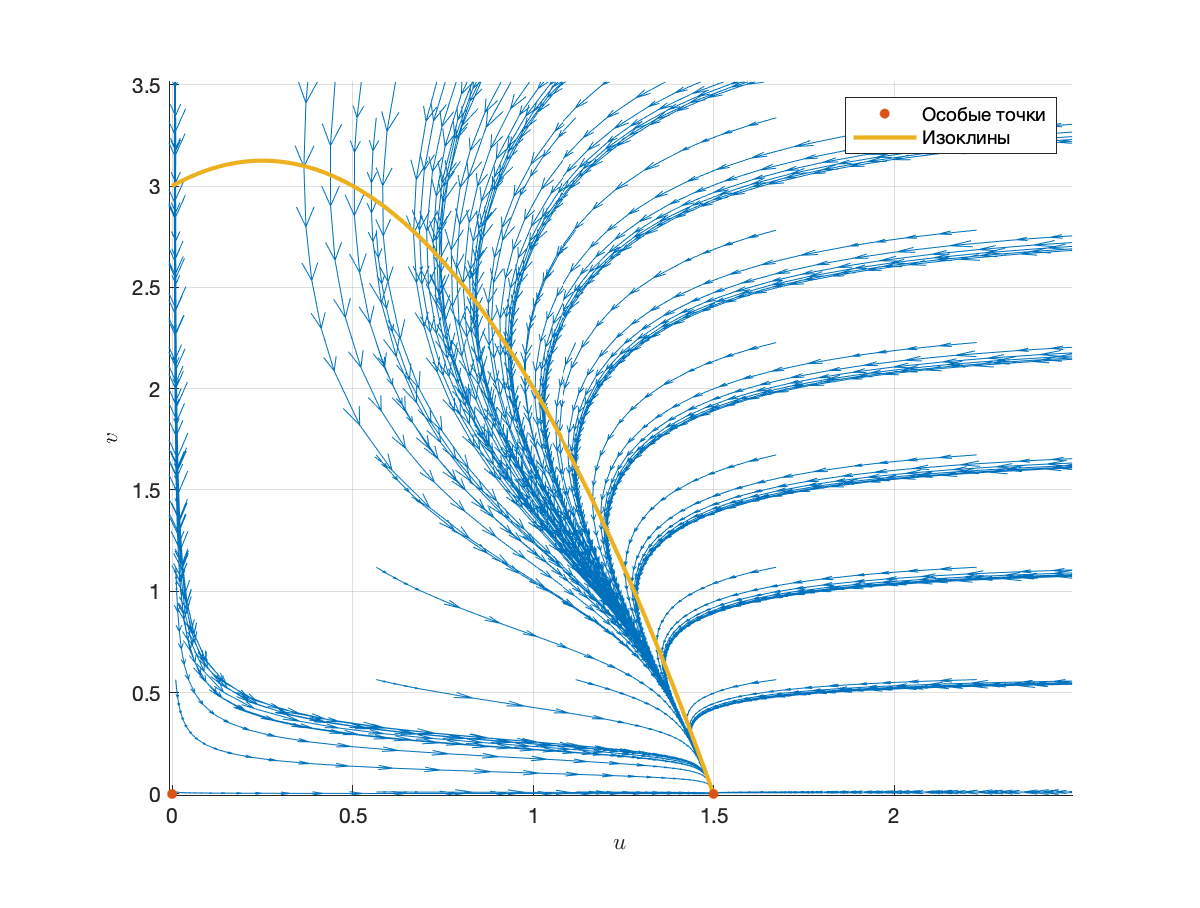
\includegraphics[width=0.45\linewidth]{schema/all_1.eps}
		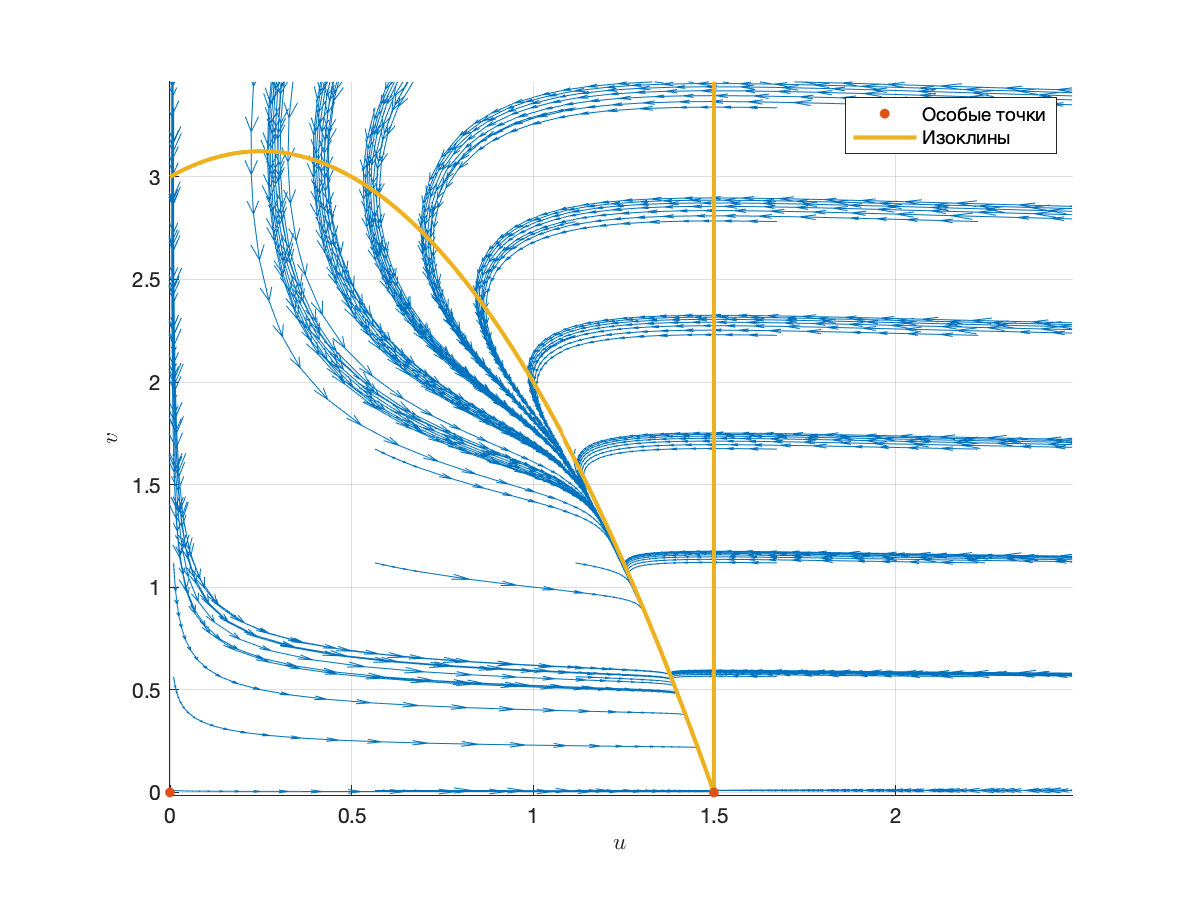
\includegraphics[width=0.45\linewidth]{schema/all_2.eps}
		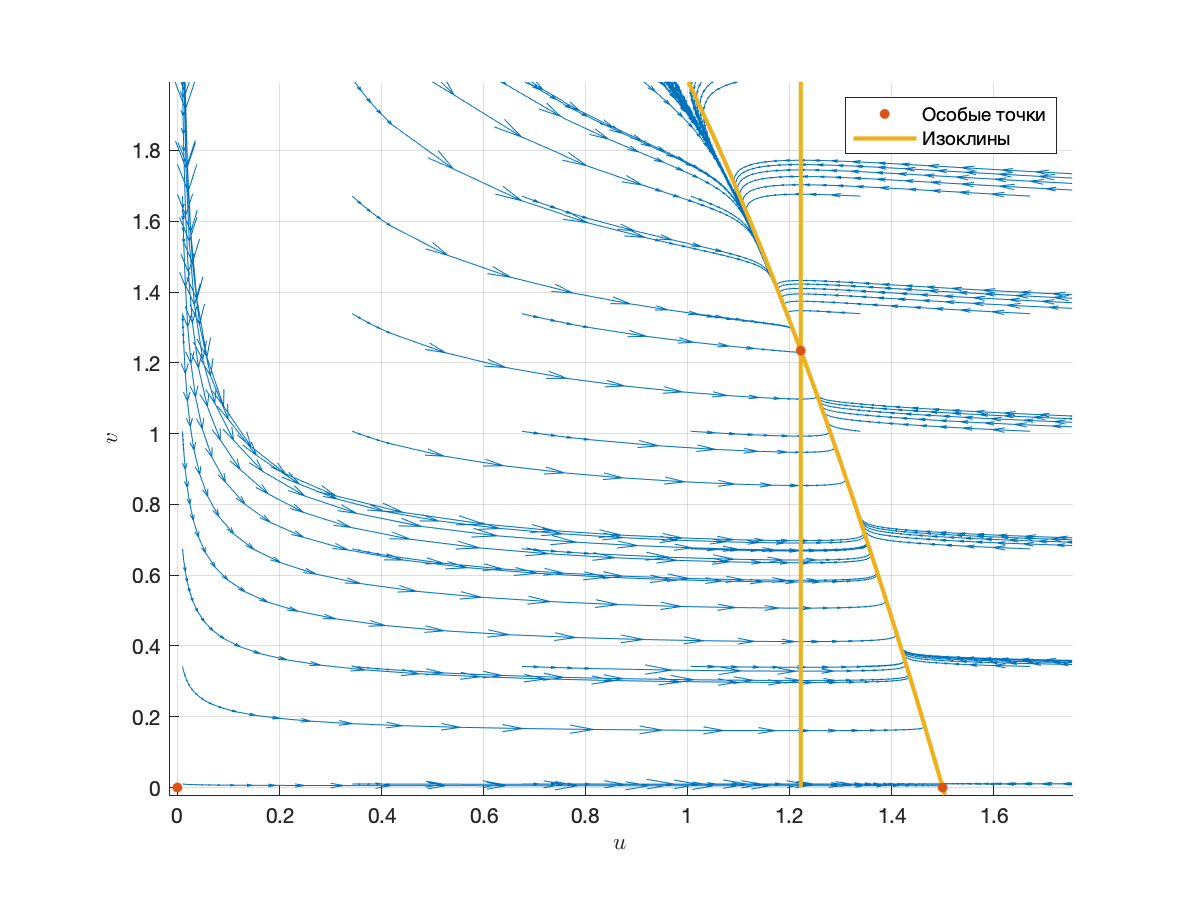
\includegraphics[width=0.45\linewidth]{schema/all_3.eps}
		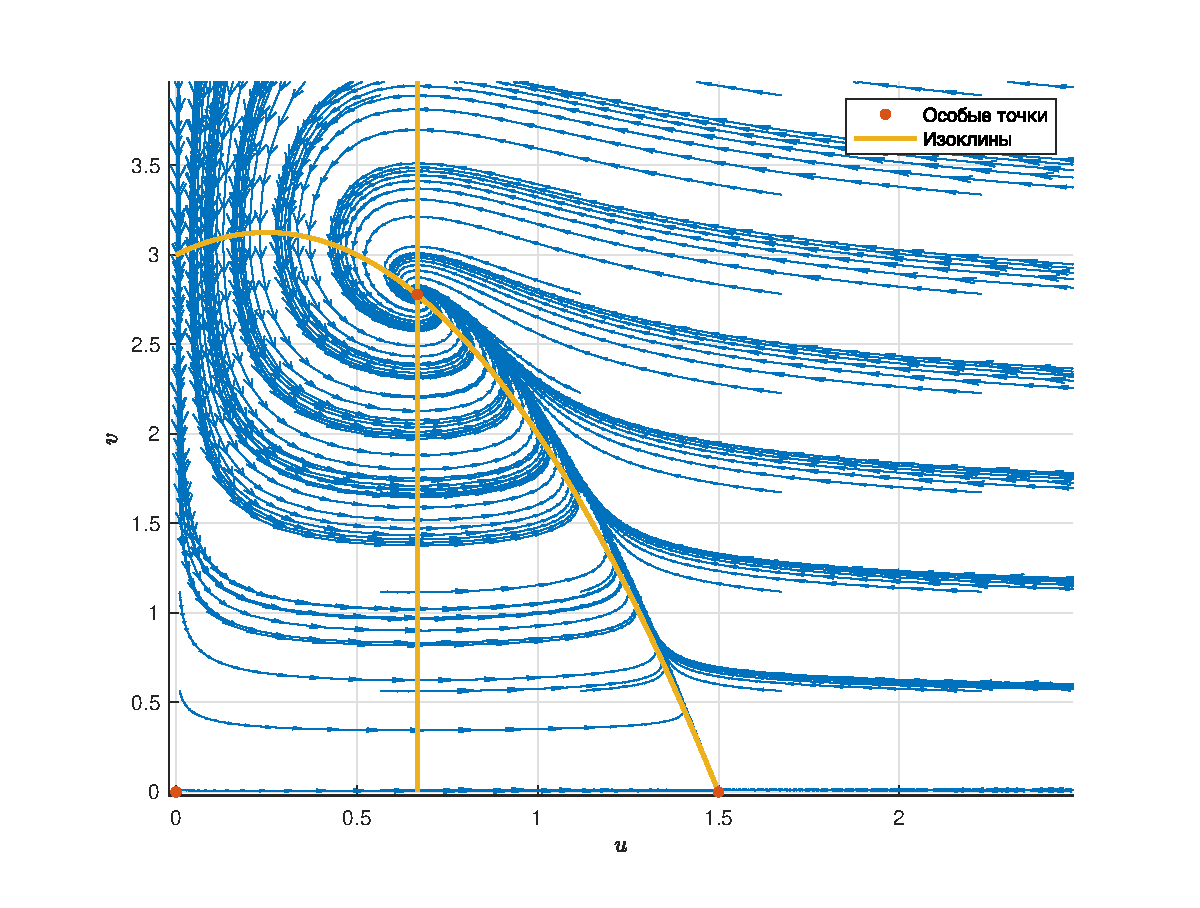
\includegraphics[width=0.45\linewidth]{schema/all_4.eps}
		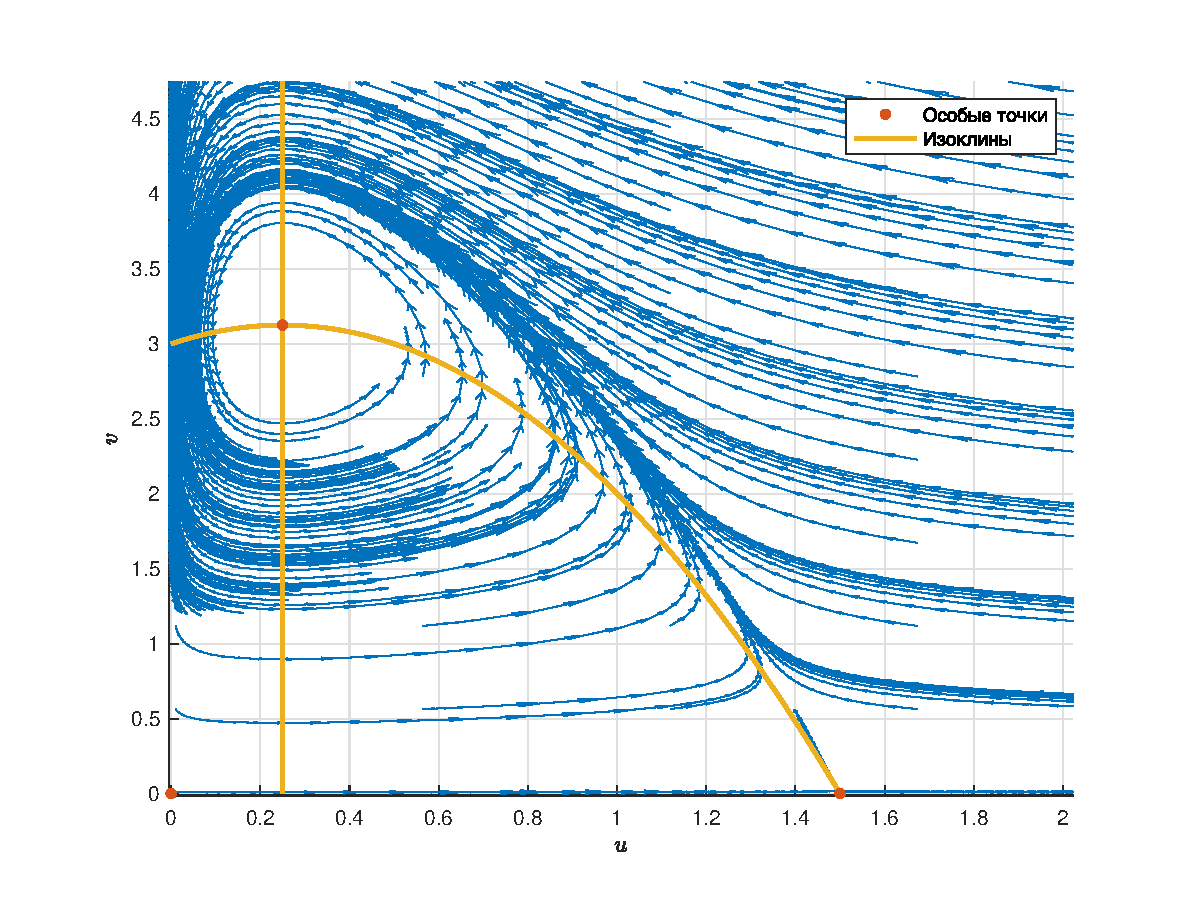
\includegraphics[width=0.45\linewidth]{schema/all_5.eps}
		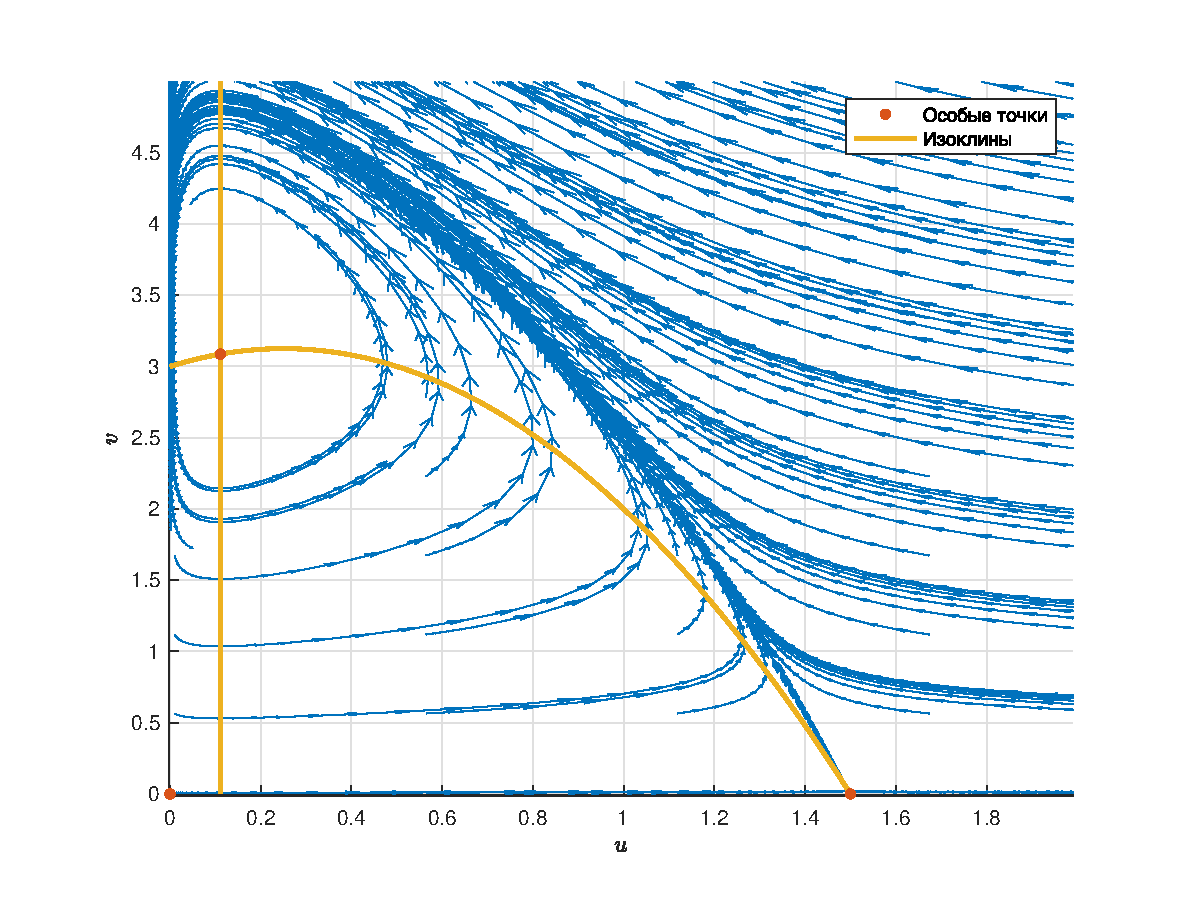
\includegraphics[width=0.45\linewidth]{schema/all_6.eps}
		\caption{Фазовые портреты всех состояний системы. Здесь были взяты фиксированные параметры $A = 2$, $B = 3$ и уменьшали $C$ от $1$ до $0,\!1$.}
	\end{figure}
	\clearpage


	\section{Исследование распределённой системы}
	Предположим, что решения системы \eqref{eq:main-task} представляются в виде $u(z) = u(x, t)$, $v(z) = v(x, t)$, $z = x + mt$, $m > 0$. Тогда система \eqref{eq:main-task} переходит в систему обыкновенных дифференциальных уравнений второго порядка:
	\begin{equation}\label{eq:base-distr-task}
		\left\{\begin{aligned}
		m u'(z) &= -Au^2(z) + Bu(z) - \frac{u(z)v(z)}{1 + u(z)} + u''(z)\\
		m v'(z) &= -Cv(z) + \frac{u(z)v(z)}{1 + u(z)} + Dv''(z)
		\end{aligned}\right.
	\end{equation}
	Упростим задачу, полагая $D = 0$, то есть считаем, что коэффициент диффузии жертв много больше, чем коэффициент диффузии хищников. При сделанных предположениях из \eqref{eq:base-distr-task} следует, что
	\begin{equation}\label{eq:distr-task}
		\left\{\begin{aligned}
		\dot u &= w \\
		\dot v &= -\frac{C}{m}v + \frac{uv}{m(1 + u)} \\
		\dot w &= Au^2 - Bu + \frac{uv}{1 + u} + mw
		\end{aligned}\right.
	\end{equation}
	В фазовом пространстве $(u, v, w)$ имеются следующие положения равновесия системы~\eqref{eq:distr-task}:
	$$
		P_1 = (0,\,0,\,0),\quad
		P_2 = \left(\frac{B}{A},\, 0,\,0\right),\quad
		P_3 = \left(\frac{C}{1-C},\,\frac{B - (A+B)C}{(1-C)^2},\,0\right).
	$$

	Исследуем устойчивость точек $P_1$, $P_2$ и $P_3$ аналогично предыдущему разделу. Матрица Якоби имеет вид:
	$$
		J(u,v,w) = \mathrm{det}\begin{pmatrix}
			-\lambda & 0 & 1 \\
			\frac{v}{c(1 + u)^2} & -\frac{C}{m} + \frac{u}{m(1+u)} -\lambda & 0 \\
			2Au - B + \frac{v}{(1+u)^2} & \frac{u}{1+u} & m -\lambda
		\end{pmatrix}.
	$$

	Рассмотрим первую точку:
	$$
		J_1 = \left(-\frac{C}{m} - \lambda\right)\left( -\lambda(m - \lambda) + B\right)
	$$
	$$
		\begin{aligned}
			\lambda_1 &= -\frac{C}{m} < 0, \\
			\lambda_{2,3} &= \frac{m \pm \sqrt{m^2 - 4B}}{2},\; \mathrm{Re}\,\lambda_{2,3} > 0.
		\end{aligned}
	$$
	Отметим, что при $m < 2\sqrt{B}$ возникают неустойчивые периодические колебания системы относительно точки $P_1 = (0,0,0)$. Так как по смыслу задачи функции $u$, $v$ неотрицательны, то этот случай необходимо исключить из рассмотрения.

	Рассмотрим вторую точку:
	$$
		J_2 = \left(-\frac{C}{m} + \frac{B}{(A+B)m} - \lambda\right)\left(-\lambda(m - \lambda)-B\right).
	$$
	$$
		\begin{aligned}
			\lambda_1 &= -\frac{C}{m} + \frac{B}{(A+B)m},\\
			\lambda_{2,3} &= \frac{m \pm \sqrt{m^2 + 4B}}{2},\; \lambda_2 > 0,\; \lambda_3 < 0.
		\end{aligned}
	$$
	Отметим, что $\lambda_1 > 0$ при $C < \frac{B}{A+B}$ и $\lambda_1 < 0$ при $C > \frac{B}{A+B}$. Все собственные значения вещественные.

	Из предыдущего следует, что при $m > 2\sqrt{B}$ и $C < \frac{B}{A+B}$ существует монотонное волновое решение, переводящее из точки $P_2$ в точку $P_1$ волновые решения; при $m > 2\sqrt{B}$ и $C > \frac{B}{A+B}$ существует монотонное волновое решение, переводящее из $P_1$ в $P_2$, либо наоборот. Приведём ниже соответствующие графики для второго случая. Из фазового портерта системы можно получить, что при любом из таких решений $v(z) \equiv 0$, что протеворечит условию задачи.

	Рассмотрим третью точку:
	$$
		J_3 = -\lambda^3 +m\lambda^2 - \frac{AC - BC + AC^2 + BC^2}{1 - C}\lambda + \frac{B - AC - BC}{m}C.
	$$
	$$
		-3\lambda^2 +2m\lambda - \frac{AC - BC +AC^2 + BC^2}{1-C} = 0.
	$$
	$$
		\lambda_{\mathrm{max}, \mathrm{min}} = \frac{-m \pm \sqrt{m^2 + 3\frac{AC-BC+AC^2+BC^2}{1 - C}}}{-3}.
	$$
	Из последнего соотношения вытекает, что либо существует как минимум одно вещественное собственное значение с положительной действительной частью, либо существует два комплексно-сопряженных собственных значения с положительной действительной частью.

	Из анализа нераспределённой системы мы ожидаем, что при близости к $C$ к $\frac{B}{A+B}$ мы будем иметь монотонный переход из $P_3$ в $P_1$, а при близости  $С$ к нулю не обязательно монотонный переход. Приведем графики для второго случая как более интересного.

	Приведём изоклины данной системы:
	$$
		\begin{aligned}
			u &= \frac{1}{1-C},\\
			v &= -\frac{A}{m}u^2 + \frac{B}{m}u - \frac{uv}{m(1+u)},\\
			w &= 0.
		\end{aligned}
	$$

	\clearpage
		\begin{figure}[t]
			\centering
			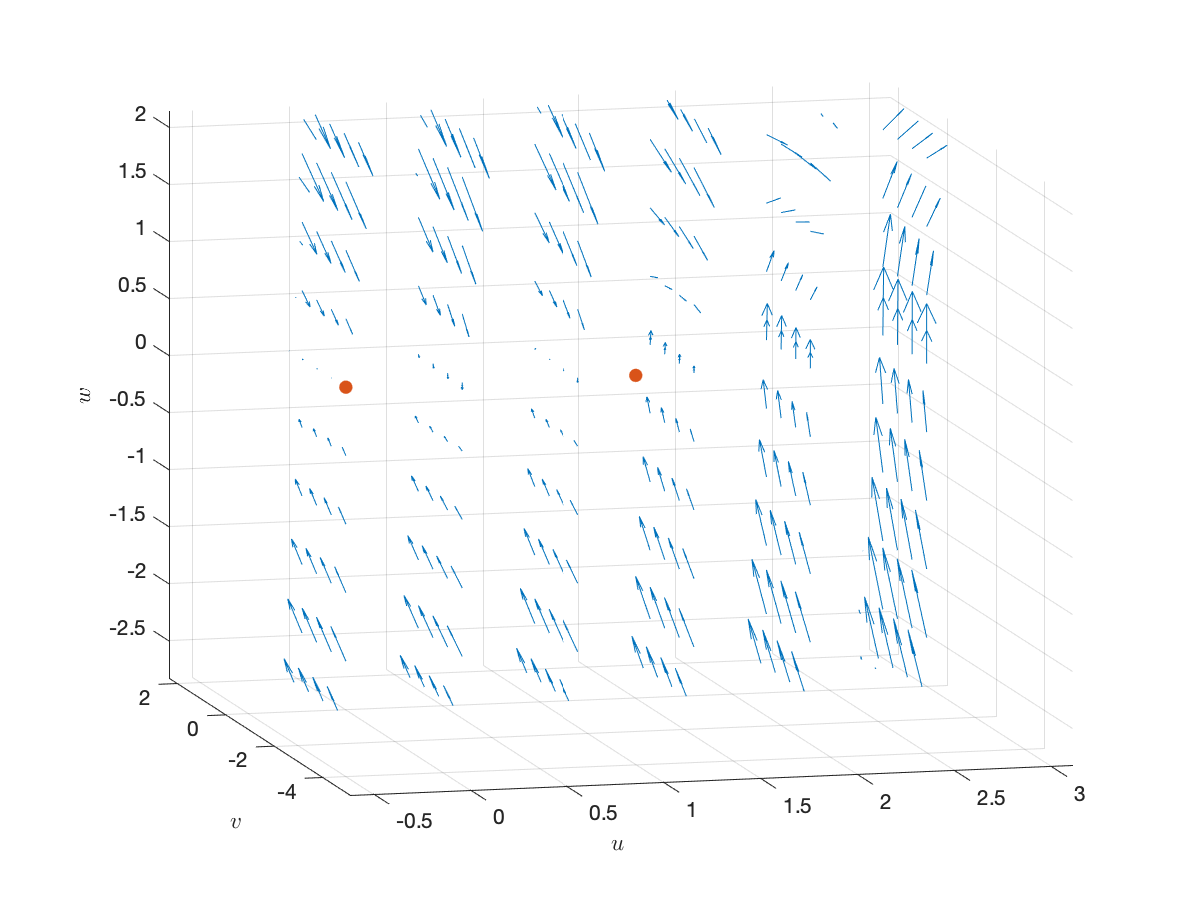
\includegraphics[width=0.45\linewidth]{p2p1-portret.eps}
			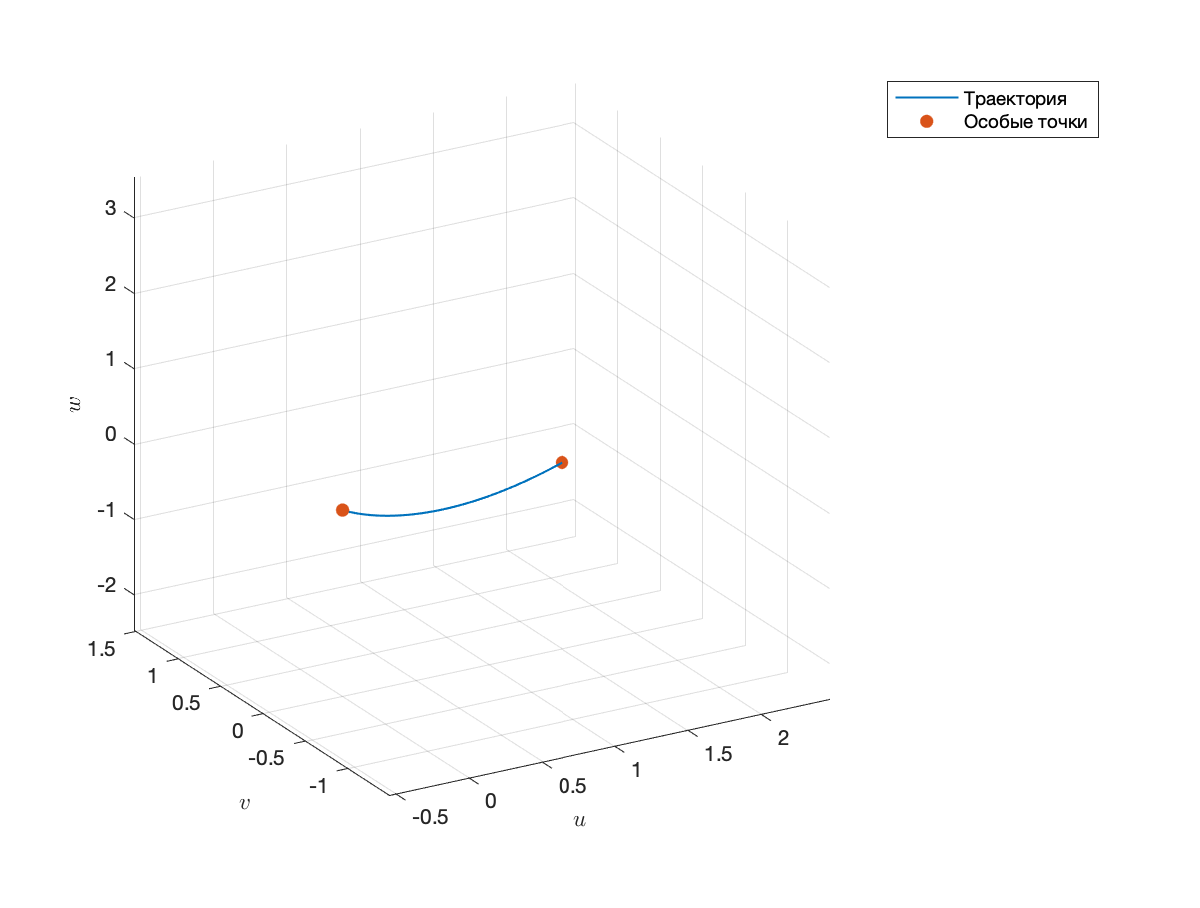
\includegraphics[width=0.45\linewidth]{p2p1-traectory.eps}
			\caption{Фазовый портрет системы \eqref{eq:distr-task} вблизи точки при $A=2,\,B=3,\,C=2,\,m=4$ и траектория волнового решения.}
		\end{figure}
		\begin{figure}[t]
			\centering
			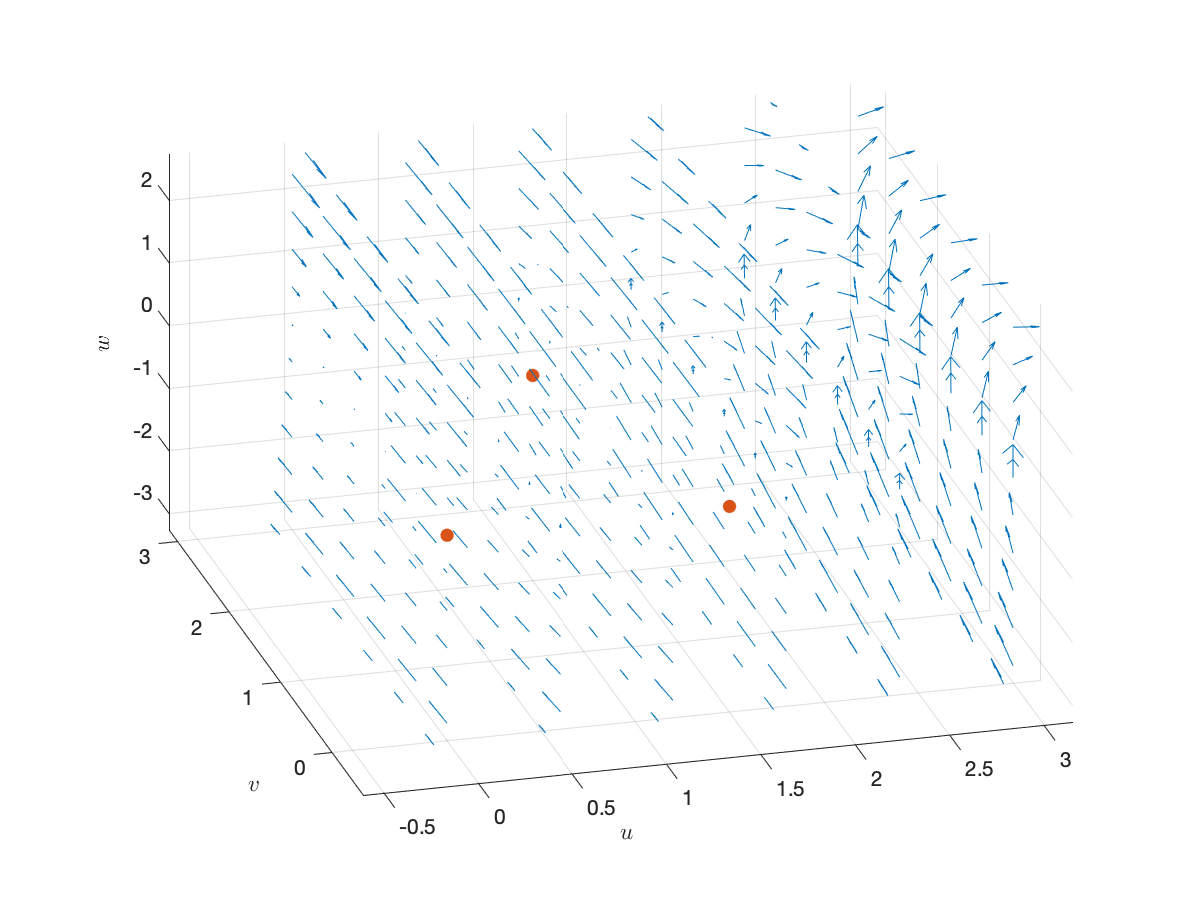
\includegraphics[width=0.45\linewidth]{p3p1-portret.eps}
			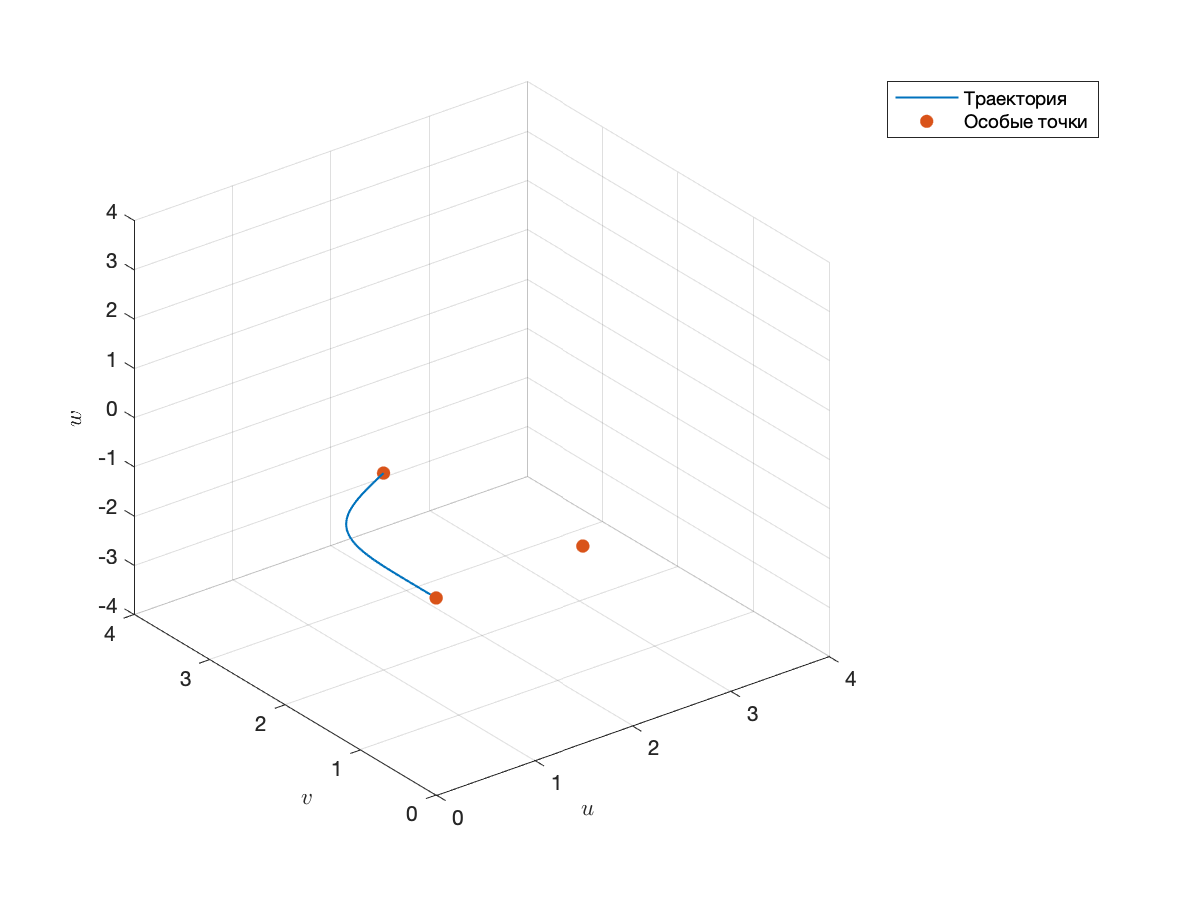
\includegraphics[width=0.45\linewidth]{p3p1-traectory.eps}
			\caption{Фазовый портрет системы \eqref{eq:distr-task} вблизи точки при $A=2,\,B=3,\,C=0,\!5,\,m=4$ и траектория волнового решения.}
		\end{figure}
		\begin{figure}[t]
			\centering
			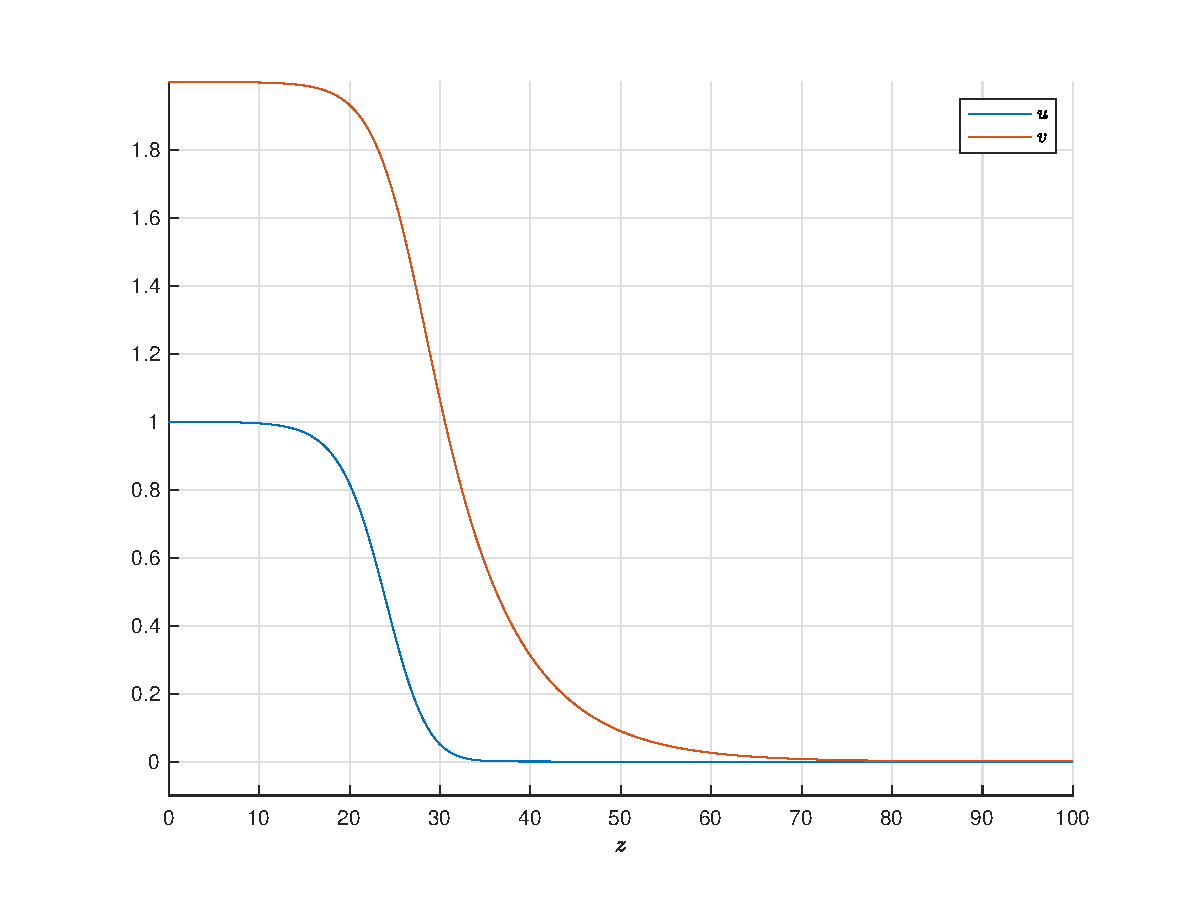
\includegraphics[width=0.7\linewidth]{p3p1-uv.eps}
		\end{figure}
		\begin{figure}[t]
			\centering
			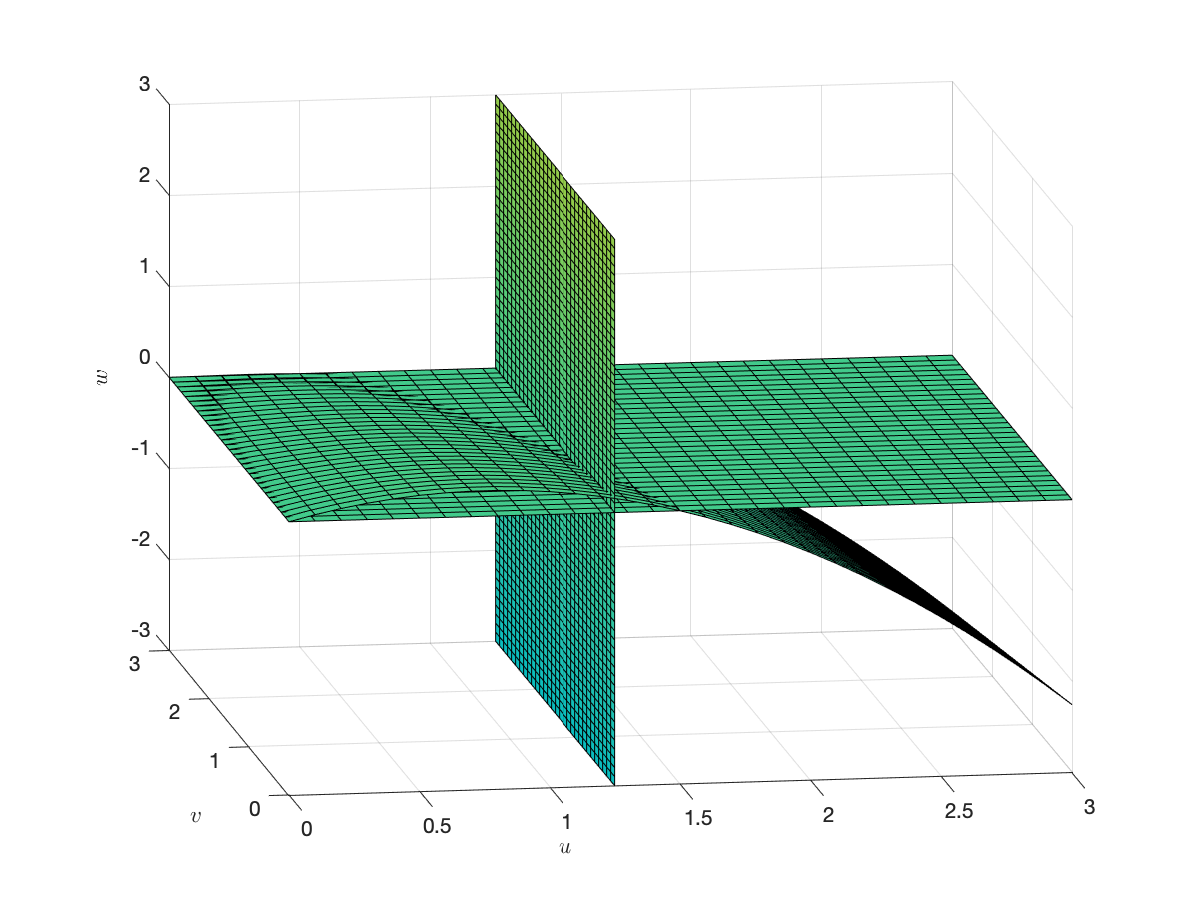
\includegraphics[width=0.7\linewidth]{izo.eps}
			\caption{Изоклины системы \eqref{eq:distr-task}.}
		\end{figure}
	\clearpage
	\begin{thebibliography}{9}
                \bibitem{bratus10} А.~С.~Братусь, А.~С.~Новожилов, А.~П.~Платонов. Динамические системы и~модели биологии. М.: ФИЗМАТЛИТ, 2010.
    \end{thebibliography} 
\end{document}